\documentclass[a4paper, 10pt]{ctexart} %中文支持
\usepackage{float}              %防止浮动元素浮动
\usepackage{rotating}           %旋转图片用的
\usepackage[]{amsmath}          %数学公式
\usepackage{amsfonts}           %加载数学字体, 比如说\mathbb, 没有这个宏包的话可能会报错
\usepackage{amsthm}             %定义, 定理, 证明, 例子这些环境的支持
%使用方法:
%\newtheorem{environment name}{caption}
%比如 \newtheorem{example}{这是例子}
%效果 \begin{example} xxx \end{example} -> 这是例子 1 xxx
%proof就不需要了
\usepackage{graphicx}           %用来插入图片
\usepackage[left=1.25in,right=1.25in,top=1in,bottom=1in]{geometry}   %用来排版的
\usepackage[]{color}            %用来给部分文本上色的
\usepackage{algorithm}          %用来写伪代码的
\usepackage{algorithmic}        %同上
\usepackage{minted}
\usepackage{extarrows}
%以下是宏包 amsthm 的命令, 我们使用这些环境的时候必须先对其进行一个定义

\newtheorem{theorem}{定理}
\newtheorem{example}{Example}
\newtheorem{definition}{Definition}
\newtheorem{lemma}{Lemma}
\title{算法第四章作业}
\author{210110531 \and 毛翰翔}
\date{\today}
\begin{document}
\maketitle
1. 
在一条直线上有n堆石子,每堆有一定的数量,每次可以将两堆相邻的石子合并,合并后放在两堆的中间位置,合并的费用为两堆石子的总数。求把所有石子合并成一堆的最小花费(定义dp[i][j]为第i堆石子到第j堆合并的最小花费)。

(1)写出该问题的递推方程。(10分)

(2)有5堆石子(n=5),每堆石子大小分别为<1,3,5,2,4>,求出把所有石子合并成一堆的最小花费(要求写出运算矩阵)。(10分)

(3)写出该问题的伪代码。(10分)


(1) : 
记 $n \left[ i \right]$ 是第 $i$ 堆石头的数量, 并且 $weight \left[  i \right] \left[ j \right]$ 是 $i$ 到 $j$ 的石头数量之和. 

有: 
\[
\text{dp}[i][j]  = 
\begin{cases}
    0 & i = j \\ 
    \min_{i \le k \le j-1} \left\{\text{dp}[i][k] + \text{dp} [k+1] [j]\right\} + weight [i][j]
\end{cases}
\]

(2) :
\[
    \begin{array}{c | c c c c c}
        & 1&2&3&4&5
        \\ 
        \hline 
        1& 0 & 4 & 13 & 22 & 34 \\ 
        2& & 0 & 8 & 17 & 28 \\ 
        3& & & 0 & 7 & 17 \\ 
        4& & & & 0 & 6 \\ 
        5& & & & & 0 \\
    \end{array}
\]
所以答案是34

(3)

\begin{minted}[mathescape, 
                   linenos, 
                   numbersep=5pt,
                   gobble=2,
                   frame=lines,
                   framesep=2mm]{c++}
    int dp () {
        for (int i = 1 ; i <= n ; i++) {
            dp [i][i] = 0;
        }
        // 
        min = +infty;
        for (int i = 1; i <= n ;i++) {
            for (int j = i ; j <= n ; j ++){
                if (i != j) {
                    for (int k = i ; k <= j -1 ;k++)
                    if (dp[i][k] + dp[k+1][j] < min)
                        min = dp[i][k] + dp[k+1][j];
                    dp[i][j] = min + weight [i][j];
                }
            }
        }
        printf("%d", dp[1][n]);
    }
\end{minted}

2. 若7个关键字的概率如下所示,求其最优二叉搜索树的结构和代价,要求必须写出递推方程。



\[
e \left[ i , j  \right] =
\begin{cases}
    \min _{i \le r \le j} \left\{e \left[  i ,r -1  \right]+ e \left[ r+1 , j \right] + w[i,j]\right\} & i +1 \ne j\\
    q_{i-1} & i +1 = j\\ 
\end{cases}
\]

代价是 3.12
\begin{figure}[H]
    \centering
    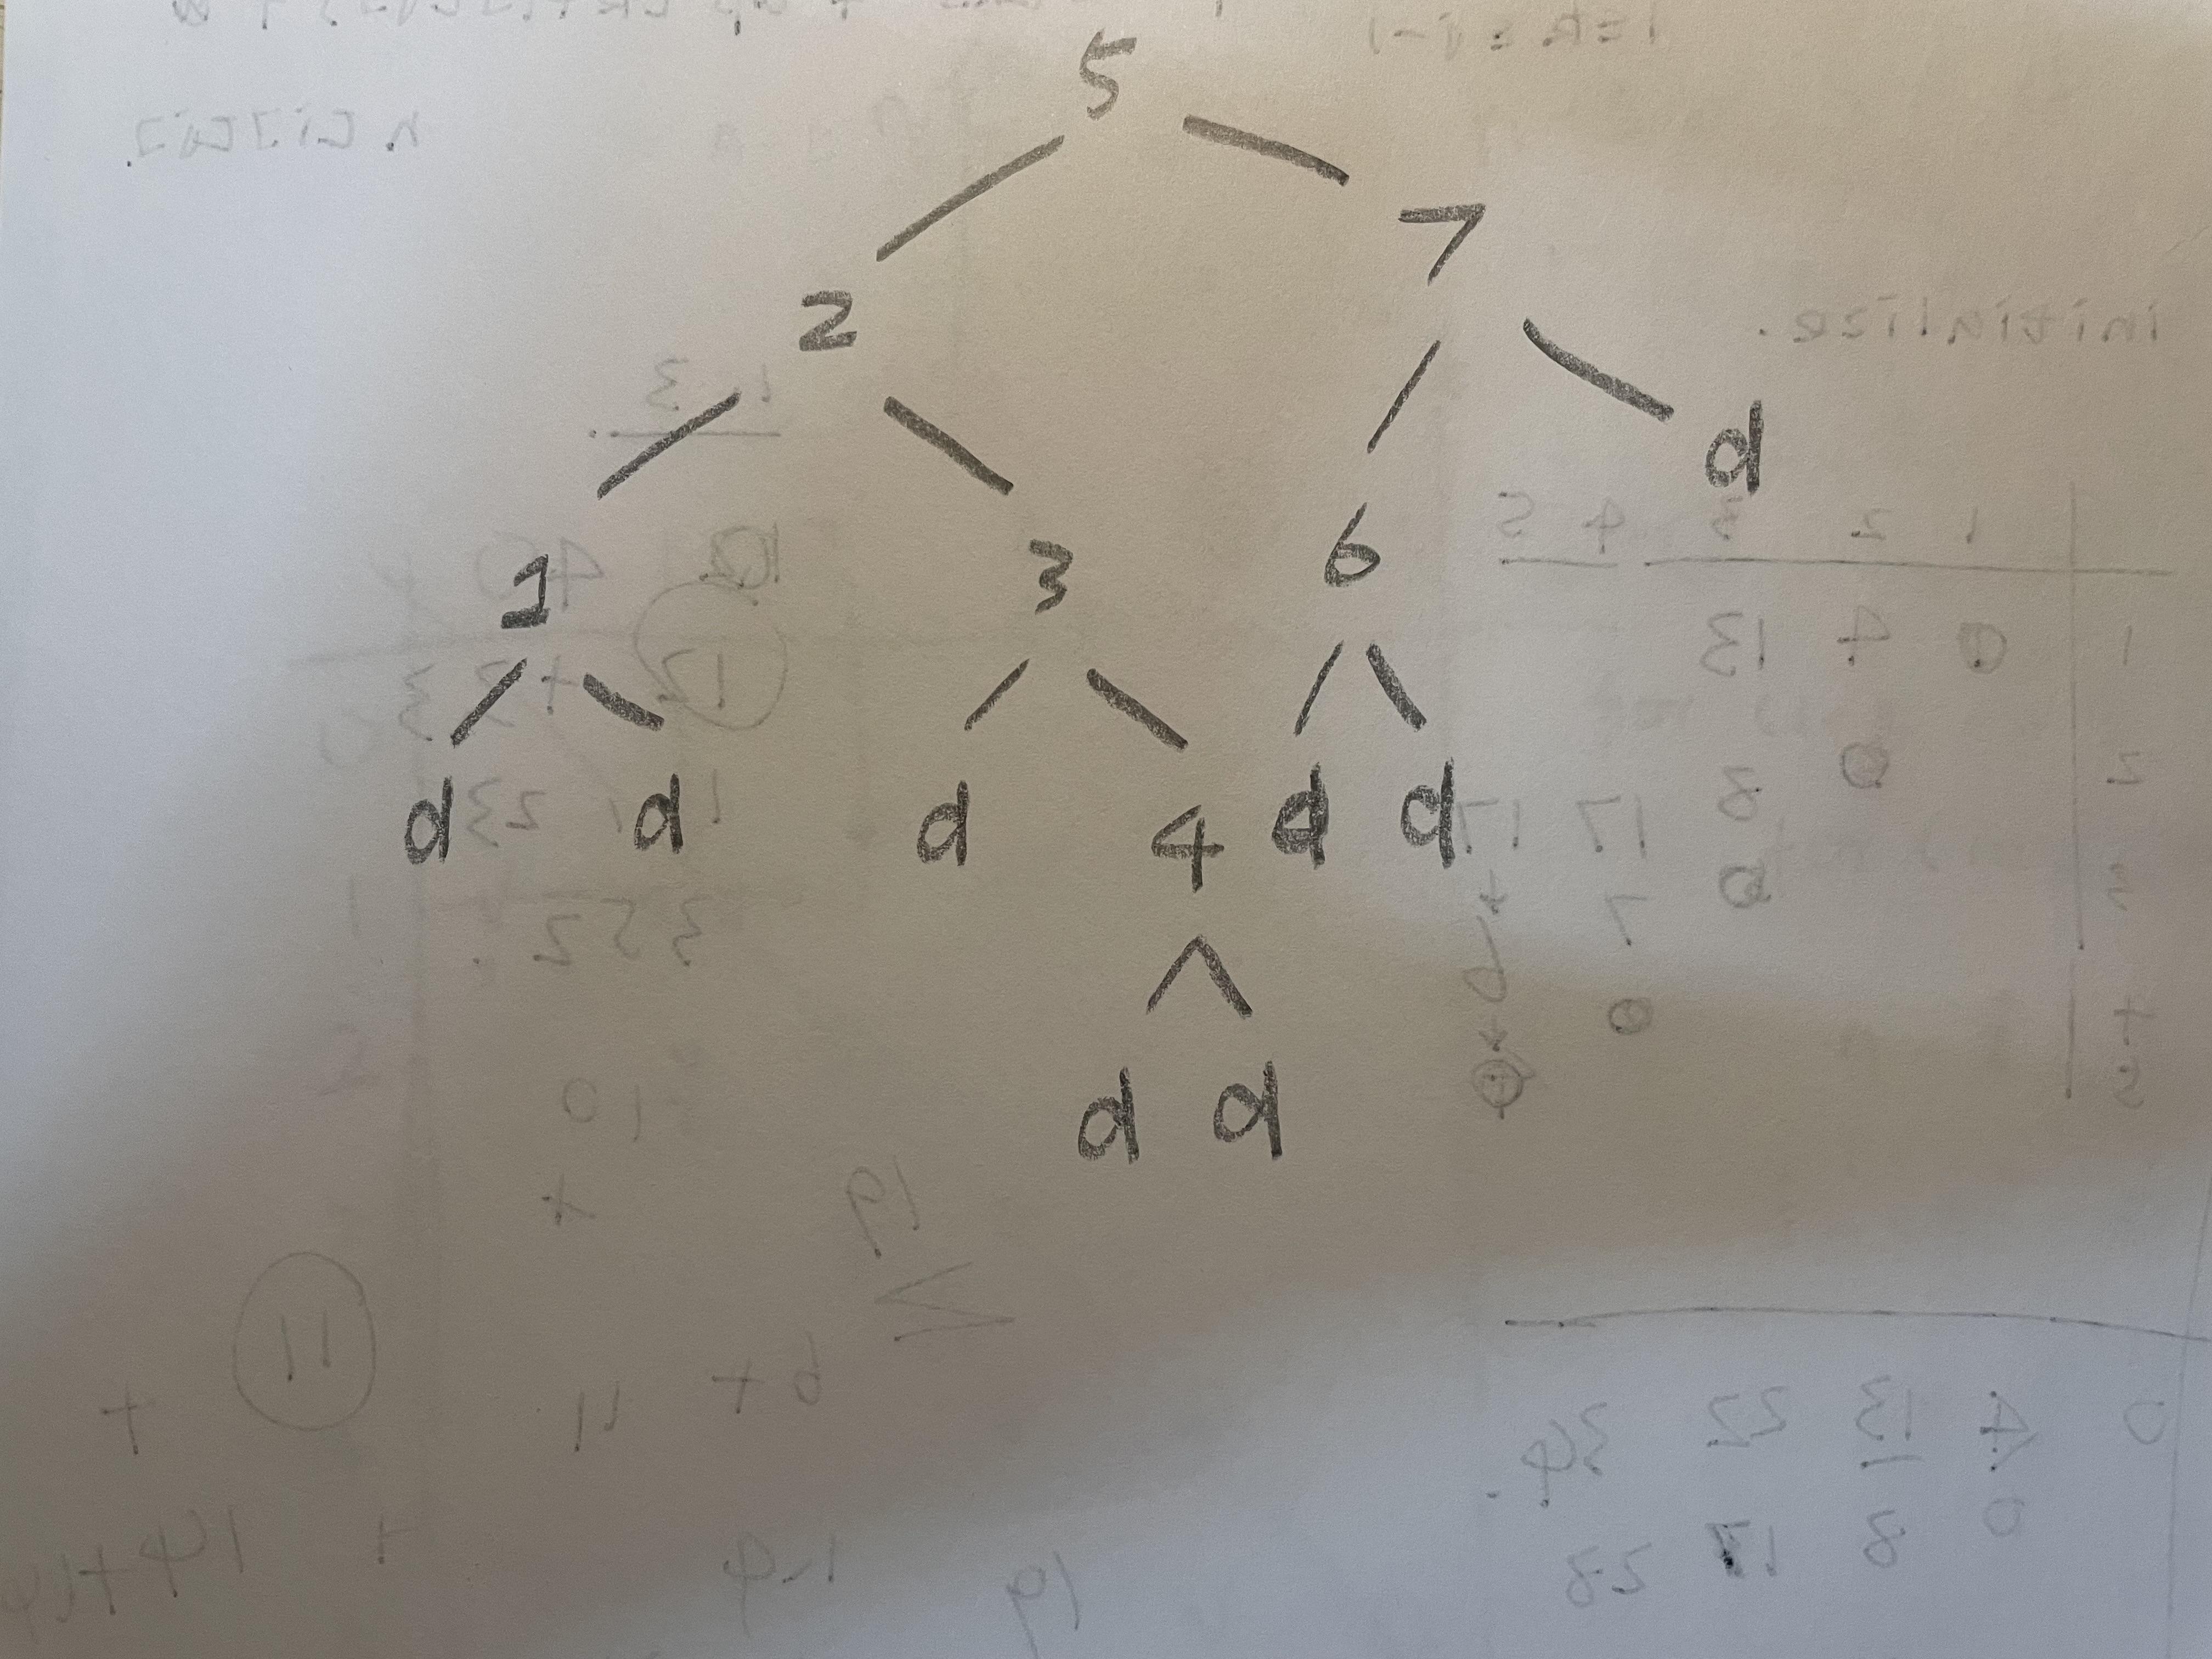
\includegraphics[scale = 0.5]{IMG_3026.jpg}
\end{figure}
\begin{minted}[mathescape, 
                   linenos, 
                   numbersep=5pt,
                   gobble=2,
                   frame=lines,
                   framesep=2mm]{c++}
    #include <stdio.h> 
    #include <stdlib.h>
    #define infty 1000
    int main (){
        int n =0;
        // n for 节点的数目, 有两组概率
        scanf ("%d", &n);
        // p q 我们说对于 n 个节点, 将会访问到 p[n]
        // 于是分配空间的时候, 必须要多一位
        int * p = (int *) malloc ( (n+1) * sizeof (int));
        int * q = (int *) malloc ( (n+1) * sizeof (int));
        // 这里就是多了一位
        // 我们的概率都是百分之几的, 我直接使用int储存了
        for (int i = 1 ; i < n + 1 ; i++) {
            scanf ("%d", &p[i]);
        }
        for (int i = 0 ; i < n+1 ; i++) {
            scanf ("%d", &q[i]);
        }
        // 这里就是读入数据.

        int e[10][10] = {}, w[10][10] = {}, root[10][10] = {};
        for (int i = 0 ; i < 10 ; i++){
            for (int j = 0 ; j < 10;j++){
                e[i][j] = 0 ; 
                root[i][j] = 0;
                w[i][j] = 0;
            }
        }
        
        // 将两个数组初始化
        for (int i = 1 ; i <= n + 1; i++){
            e[i][i-1] = q[i-1];
            w[i][i-1] = q[i-1];
        }
        // 处理最底的情况. 
        for (int i = 1 ; i < n+1 ;i++){
            for (int j = 1 ; j <= n - i + 1 ; j++){
                // i for 一种偏移量, 就是说我们是从对角线开始这样计算的, i 就是往右边便宜的程度. 
                int min = infty;
                w[j][j+i-1] = w[j][j+i-2] + p[j+i-1] + q[j+i-1];
                // 为 w 赋值. 
                for (int r = j ;r <= j+i -1 ; r++){
                // 开始找出最小值
                    if (e[j][r-1] + e[r+1][j+i-1] + w[j][j+i-1] < min) {
                        min = e[j][r-1] +  e[r+1][j+i-1] + w[j][j+i-1];
                        root[j][j+i-1] = r;
                    }
                }
                e[j][j+i-1] = min;
            }
        }
        printf("%d\n", e[1][n]);
        // 这就是结果了
    }
\end{minted}

3. 编程题:兑换零钱问题(40分)\\
题目描述:\\
给定不同面额的硬币 coins 和一个总金额 amount。编写一个函数来计算可以凑成总金额所需的最少的硬币个数。如果没有任何一种硬币组合能组成总金额,返回-1。(提示:你可以认为每种硬币的数量是无限的)。

首先分析优化解的结构, 类似的, 我们用矩阵 $dp$ 来记录最优解, 其中第一个指标指的是使用的硬币的种类, 第二指标是指总额. 硬币的种数按照升序排列, 就是说 $n$ 种硬币指 前 $n$ 个面值最小的硬币.
于是我们可以将问题划分为几个子问题
\\ 如果说当前 $i$ 硬币并没有使用, 那么问题的解就是 $dp[i-1][j]$, 如果说当前 $i$ 硬币使用了 $k$ 个, 那么问题的解是 $dp[i-1][j-k v_i] + k$

就有: 
\[
dp[i][j] = \min_{1 \le k \le \left\lfloor j / v_i \right\rfloor} \left\{ dp [i-1]\left[ j \right], dp [i-1][j - k v_i] + k \right\}
\]

接着定义最初的解: 当种数为 $1$ 的时候. 如果说不能凑出来, 则 $j \text{ mod } v_1 \ne 0$ , 此时定义 $dp[1][j] = +\infty$. 
问题就能解决了. 最后如果 $dp [n][ \text{amount}]$ 是正无穷的话, 则说明不能凑出来, 返回 $-1$ 即可

综上就是:
\[
dp\left[ i \right]\left[ j \right] = 
\begin{cases}
    0 & j = 0\\
    \displaystyle j / v_i& i = 1, j \text{ mod } v_i = 0\\
    \displaystyle +\infty & i = 1, j \text{ mod } v_i \ne 0 \\
    \displaystyle \min _{1 \le k \le \left\lfloor j / v_i \right\rfloor} \left\{ dp \left[ i-1 \right] \left[ j \right] , dp \left[ i-1\right]\left[ j-k v_{i}   \right] +k\right\} & i \ne 1
\end{cases}
\]

\begin{minted}[mathescape, 
                   linenos, 
                   numbersep=5pt,
                   gobble=2,
                   frame=lines,
                   framesep=2mm]{c++}
    #define infty 10000
    int main (){
        int n =0, amount = 0, min = infty;
        scanf("%d %d", &n, &amount);
        // 读取 n amount
        int ** dp = (int **) malloc (n*amount * sizeof (int));
        int * v = (int *) malloc ((n+1) * sizeof (int));
        // 分配矩阵 dp 和向量 v
        // 分别储存最优解, 和每种硬币的面额

        for (int i = 1 ; i <= n ; i++){
            scanf ("%d" , &v [i]);
        }
        // 读取面额

        for (int i = 1; i <= n ; i++){
            dp[i][0] = 0;
        }
        // amount 为 0 的时候的初始化. 
        for (int i = 1 ; i <= amount ; i++){
            if (i % v[1] != 0)
            dp[1][i] = infty;
            else 
            dp[1][i] = i / v[1];
        }
        // 只使用了一种硬币的情况. 
        for (int i = 2 ; i <= n ; i++){
            for (int j = i ; j<= amount ; j++){
                // 开始处理一般矩阵的成员
                min = dp[i-1,j] ;
                // 先赋值, 以此避免在 v[i] > j 的情况下访问数组. 
                if (v[i] <= j){
                    for (int k = 1; k <= j / v[i]; k++){
                        // k 就是使用了硬币的个数, 从1开始计数
                        if (dp[i-1][j - k * v[i]] + k < min)
                            min = dp[i-1][j - k * v[i]] + k ;
                    }
                    dp[i][j] = min;
                    // 将最小的值放入 dp [i][j]
                }
            }
        }
        if (dp[n][amount] == infty)
            return -1;
        else 
            return dp[n][amount];
    }
\end{minted}
\end{document}